\documentclass[]{article}

\usepackage[left=1in,right=1in,top=1in,bottom=1in]{geometry}
\usepackage{amsmath,amsfonts}
\usepackage{graphicx}
\usepackage{hw}

\setlength{\parindent}{0pt}

\graphicspath{ {.} }


\begin{document}
\section*{Q1}
1. False. When the number of samples is very small, Apriori (with time complexity is $2^n$) might be faster that FP-growth (with time complexity $n^2$).

2. False. The sequence itself can be unordered. 

3. False. The support vectors lie on the margin bound. 

4. False. Most clustering methods are unsupervised. 

5. False. Zero-shot learning still need labeled data to train a classifier, which is used for classification task on unseen data labels. 

6. True. According to gSPAN, the DFS code extended from a min DFC code via right-most extension is still a minimal DFS code. 

7. SVM without slack variables always returns zero training error if it can find a solution. With Gaussian kernel to support non-linear separation, the data points can be mapped to infinite dimensional feature space. That means there is always a boundary plane that can separate the data of two classes after mapping. The solution is feasible and the training error is achieved. 

8. High intra-class similarity and low inter-class similarity. The generated clusters have high interpretability and usability. 


\newpage

\section*{Q2}
\subsection*{a}
Let $X=$hot dogs, $Y=$hamburgers,
$s(X,Y) = 2000/5000 =0.4 > 25\%$\\
$c(X\Rightarrow Y) = sup(X,Y)/sup(X)=2000/(2000+1000)=0.67 > 50\%$

So $X \Rightarrow Y$ is strong association

\subsection*{b}
Since the null transaction $(\overline{X}, \overline{Y})$ is not dominant, then lift and $\chi^2$ can be used for evaluation. 

$lift(X, Y)=\cfrac{c(X\rightarrow Y)}{s(Y)}=\cfrac{0.67}{2500/5000}=1.33>1$

The expected value of each event should be (shown in parentheses):\\
\begin{table}[!ht]
    \centering
    \begin{tabular}{c c c}
    \hline
     & \textbf{hot dogs} & \textbf{$\overline{hot dogs}$} \\
    \hline
    hamburgers & 2000 (1500) &   500(1000) \\
    $\overline{hamburgers}$ & 1000 (1500) &  1500 (1000) \\ 
    \hline
    \end{tabular}
\end{table}

$\chi^2 = \sum\cfrac{(observe-expect)^2}{expect}
=\cfrac{(2000-1500)^2}{1500}+\cfrac{(1000-1500)^2}{1500}+\cfrac{(500-1000)^2}{1000}+\cfrac{(1500-1000)^2}{1000}=833>\chi^2_{.005}$, and $observe>expect (2000>1500)$.

These measures show they X and Y are positively correlated. 

\subsection*{c}
$all\_confidence(X,Y) = \cfrac{s(X\bigcup Y)}{max\{s(X),s(Y)\}}
=\cfrac{2000}{max\{3000, 2500\}}=2000/3000=0.67$

$max\_confidence(X,Y) = max\{\cfrac{s(X\bigcup Y)}{s(X)}, \cfrac{s(X\bigcup Y)}{s(Y)}\}
=max\{2000/3000, 2000/2500\}=0.8$

$Kulczynski(X,Y)=\cfrac{1}{2}(\cfrac{s(X,Y)}{s(X)}+\cfrac{s(X,Y)}{s(Y)})
=\cfrac{1}{2}(2000/3000+2000/2500)=0.73$

$consine(X,Y)=\cfrac{s(X\bigcup Y)}{\sqrt{s(X)\times s(Y)}}
\cfrac{2000}{\sqrt{3000*2500}}=0.73$

$lift(X,Y)=1.33$

\newpage

\section*{Q3}
\subsection*{a}

With $min\_sup=0.6$, the frequent 1-itemset based on item category is: \\
\begin{table}[!ht]
    \begin{tabular}{c c c}
        \hline 
        \textbf{Itemset} & \textbf{sup} & \textbf{transaction}\\
        \hline
        Bread & 4 & \{T100, T200, T300, T400\}\\
        Milk & 4 & \{T100, T200, T300, T400\}\\
        Cheese & 3 & \{T100, T200, T400\}\\
        \hline
    \end{tabular}
\end{table}

So the 2-itemset is: \\
\begin{table}[!ht]
    \begin{tabular}{c c }
        \hline 
        \textbf{Itemset} & \textbf{sup} \\
        \hline
        \{Bread, Milk\} & 4 \\
        \{Bread, Cheese\} & 3 \\
        \{Milk, Cheese\} & 3 \\
        \hline
    \end{tabular}
\end{table}

The 3-itemset is: \\
\begin{table}[!ht]
    \begin{tabular}{c c }
        \hline 
        \textbf{Itemset} & \textbf{sup} \\
        \hline
        \{Bread, Milk, Cheese\} & 3 \\
        \hline
    \end{tabular}
\end{table}

So the largest k is 3 with 3-itemset \{Bread, Milk, Cheese\}. 

These are the strong association rules:\\
1. $\forall X\in transaction, buys(X,Bread)\wedge buys(X,Cheese)\Rightarrow buys(X, Milk)[0.75,1]$, \\
2. $\forall X\in transaction, buys(X,Milk)\wedge buys(X,Cheese)\Rightarrow buys(X, Bread)[0.75,1]$, \\

% $s(\{Bread, Cheese\}\Rightarrow Milk) = 3$\\
% $c(\{Bread, Cheese\}\Rightarrow Milk)=s(Bread\bigcap Milk\bigcap Cheese)/s(Bread\bigcap Cheese)=3/3=1> min\_conf$

\subsection*{b}
With $min\_sup=0.6$, the frequent 1-itemset based on brand-item category is: \\
\begin{table}[!ht]
    \begin{tabular}{c c c}
        \hline 
        \textbf{Itemset} & \textbf{sup} & \textbf{customer}\\
        \hline
        Wonder-Bread & 3 & \{01, 02, 03\} \\
        Dairyland-Milk & 2 & \{01, 02\} \\
        Tasty-Pie & 2 & \{01, 02\} \\
        Dairyland-Cheese & 2 & \{01, 03\} \\
        Sunset-Milk & 2 & \{01, 03\}\\
        \hline
    \end{tabular}
\end{table}

For 2-itemset,\\
\begin{table}[!ht]
    \begin{tabular}{c c c}
        \hline 
        \textbf{Itemset} & \textbf{sup} & \textbf{customer}\\
        \hline
        \{Wonder-Bread, Dairyland-Milk\} & 2 & \{01, 02\} \\
        \{Wonder-Bread, Tasty-Pie\} & 2 & \{01, 02\} \\
        \{Wonder-Bread, Dairyland-Cheese\} & 2 & \{01, 03\} \\
        \{Wonder-Bread, Sunset-Milk\} & 2 & \{01, 03\} \\
        \{Dairyland-Milk, Tasty-Pie\} & 2 & \{01, 02\} \\
        \{Sunset-Milk, Dairyland-Cheese\} & 2 & \{01, 03\}\\
        \hline
    \end{tabular}
\end{table}

For 3-itemset, \\
\begin{table}[!ht]
    \begin{tabular}{c c c}
        \hline 
        \textbf{Itemset} & \textbf{sup} & \textbf{customer}\\
        \hline
        \{Wonder-Bread, Dairyland-Milk,Tasty-Pie\} & 2 & \{01, 02\} \\
        \{Wonder-Bread, Dairyland-Cheese, Sunset-Milk\} & 2 & \{01, 03\} \\
        \hline
    \end{tabular}
\end{table}

So the largest k is 3 with 3-itemset of \{Wonder-Bread, Dairyland-Milk,Tasty-Pie\} and \{Wonder-Bread, Dairyland-Cheese, Sunset-Milk\}.  

\subsection*{(c)}
See zongfan2\_HW1\_problem3.py

\newpage

\section*{Q4}
The length-1 candidates include $<a>, <b>, <c>, <d>$.

The initial candidates that satisfy the min support: \\
\begin{table}[!ht]
    \begin{tabular}{c c }
        \hline 
        \textbf{Candidate} & \textbf{sup} \\
        \hline
        $<a>$ & 4 \\
        $<b>$ & 4 \\
        $<d>$ & 4 \\
        \hline
    \end{tabular}
\end{table}

For the length-2 candidates, they can be: $<aa>, <ab>, <ad>, <ba>, <bb>, <bd>,<da>,<db>,<dd>,<(ab)>, <(ad)>, <(bd)>$. 
The candidates that satisfy the min support include:
\begin{table}[!ht]
    \begin{tabular}{c c }
        \hline 
        \textbf{Candidate} & \textbf{sup} \\
        \hline
        $<aa>$ & 4 \\
        $<ab>$ & 3 \\
        $<da>$ & 3 \\
        \hline
    \end{tabular}
\end{table}

For the length-3 candidates, they can be: $<aaa>, <aab>, <aba>, <baa>, <aad>, <ada>, <daa>, <dab>, <abb>, <bab>, <abd>, <adb>, <bda>, <dba>, <dda>, <dad>$. 
After pruning by Apriori rule, only $<aaa>, <aab>, <daa>$ are left. 
No such frequent itemset is found that can satisfy the min support requirement.

\newpage
\section*{Q5}
With the min-support = 2, the DFS code tree looks like this: 

\begin{figure}[!ht]
    \centering
    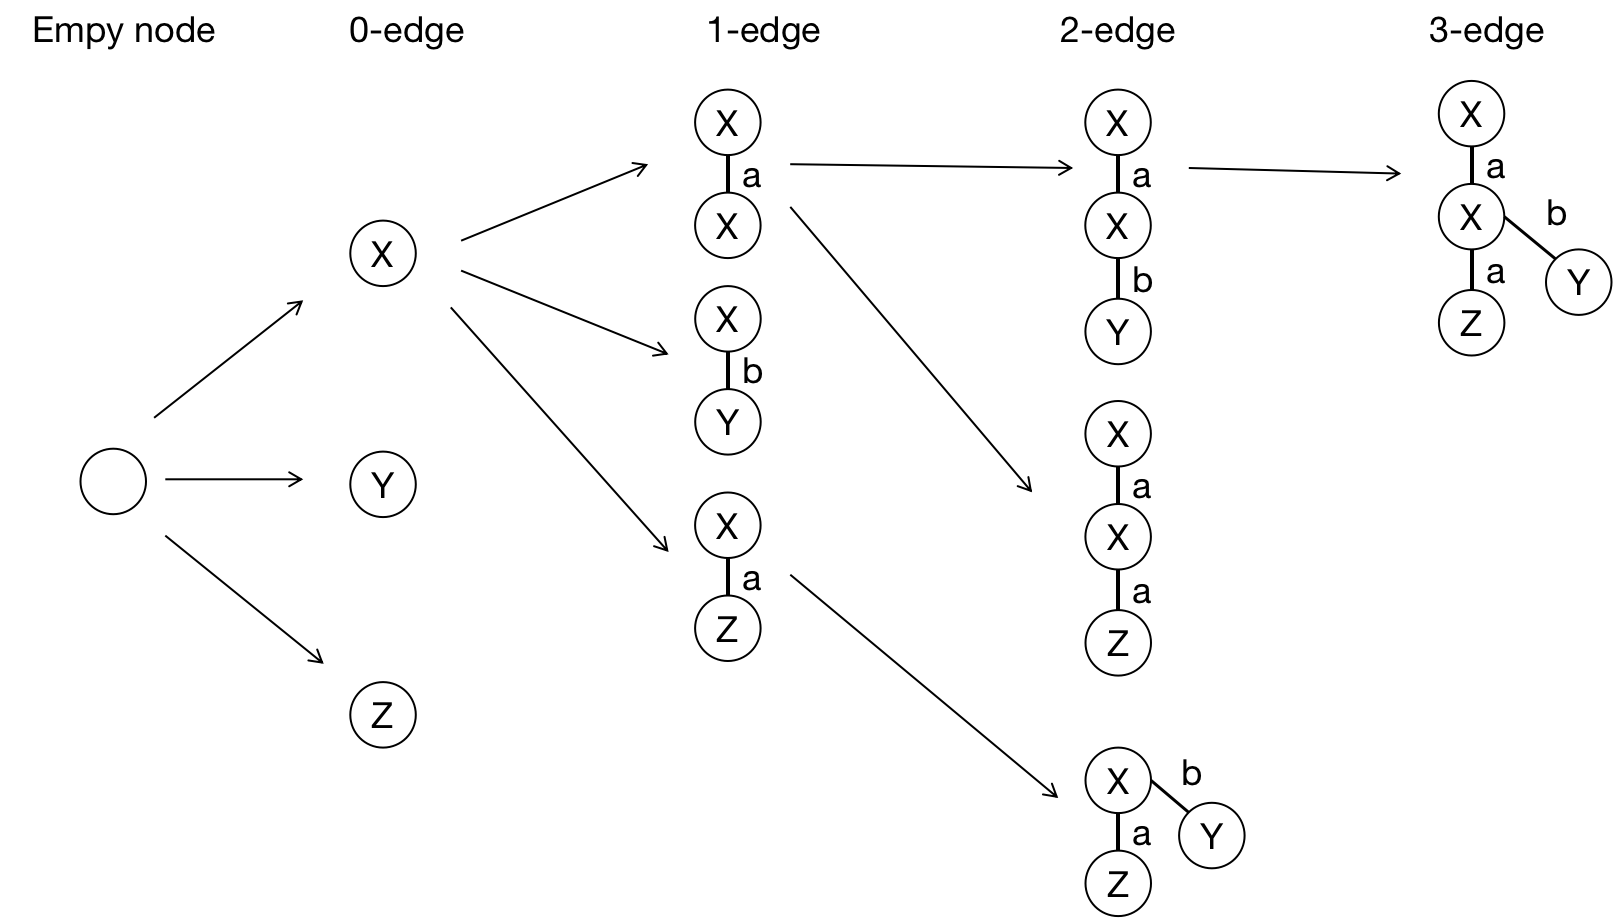
\includegraphics[width=0.8\textwidth]{fig/hw1_q5.png}
\end{figure}

\newpage
\section*{Q6}
\subsection*{(a)}
The boundaries of SVM and logistic regression (LR) in figure (a) and (b) cases look like this:\\

\begin{figure}[!ht]
    \centering
    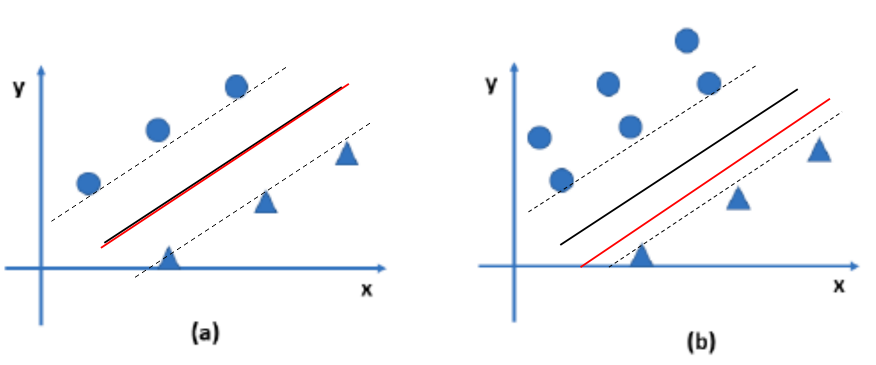
\includegraphics[width=0.8\textwidth]{fig/hw1_q6.png}
    \caption{Black solid lines represent the boundaries of SVM; Red solid lines represent the boundaries of LR.}
\end{figure}

SVM performs better on imbalanced dataset to reduce the risk of overfitting, especially when the support vectors don't change. 

\subsection*{(b)}
Loss function of soft-margin linear SVM:

$min_{w,b}\cfrac{1}{2}w^Tw+C\sum_{i=1}^m\xi_i$, \\
s.t. $y_i(w^Tx_i+b)\ge1-\xi_i,\forall i$ and $\xi_i\ge0,\forall i$

The unconstrainted form of objective function can be: $min_{w,b}\cfrac{1}{2}w^Tw+C\sum_{i=1}^mmax(1-y_i(w^tx_i+b), 0)$

Its dual form is $max_\alpha\ell(\alpha)=\sum_{i=1}^m\alpha_i-\cfrac{1}{2}\sum_{i,j=1}^m\alpha_i\alpha_jy_iy_j(\mathbf{x}_i^T\mathbf{x}_j)$, \\
s.t. $0\le\alpha_i\le C,i=1,\dots,m$ and $\sum_{i=1}^m\alpha_iy_i=0$

\vspace{0.5cm}
Loss function of logistic regression with L2-norm is: \\
$min_\theta \ell(\theta) =\cfrac{1}{m}[\sum_{i=1}^m-y^ilog(h_\theta(x^i))+(1-y^i)log(1-h_\theta(x^i))]+\cfrac{\lambda}{2m}\sum_{j=1}^n\theta_j^2$ \\
where $h_\theta(x)=\cfrac{1}{1+e^{-\theta^Tx}}$ and $\lambda$ is the constraint factor. 

Commonality: 
1. Both of them can find a linear boundary to separate the feature space and have unconstrainted smooth objective function. 

2. With regularization, both can reduce the risk of overfitting. 

Difference: 
1. LR is based on probabilistic difference of different classes but SVM is based on geometric difference. The predicted probability can be interpreted as confidence when predicting new data samples. 

2. Soft-margin SVM doesn't penalize examples in the region between boundary margins. This is good for generalization. 

3. SVM only relies on a small set support vectors to determine the decision boundary, which has nice sparsity. 

4. SVM has nice dual form and a flexible choice of kernels.

\subsection*{(c)}
Let $k_1(x_i,x_j)=\Phi_1(x_i)^T\Phi_1(x_j)$ and $k_2(x_i,x_j)=\Phi_2(x_i)^T\Phi_2(x_j)$,

$k_3(x_i,x_j)=c_1k_1(x_i,x_j)+c_2k_2(x_i, x_j)=c_1(\Phi_1(x_i)^T\Phi_1(x_j))+c_2(\Phi_2(x_i)\Phi_2(x_j))\\
% =c_1(\sum_{i=1}^n\phi_i(x_1)\phi_i(x_2))+c_2(\sum_{j=1}^n\phi_j(x_1)\phi_j(x_2))\\
=\newmat{\sqrt{c_1}\Phi_1(x_i)\\\sqrt{c_2}\Phi_2(x_i)}^T \newmat{\sqrt{c_1}\Phi_1(x_j)\\\sqrt{c_2}\Phi_2(x_j)}$

Let $\Phi_3(x)=\newmat{\sqrt{c_1}\Phi_1(x)\\\sqrt{c_2}\Phi_2(x)}$, then $k_3(x_i,x_j)=\Phi_3^T(x_i)\Phi_3(x_j)$, which is a kernel. 

\vspace{1cm}
$k_3(x_i,x_j)=k_1(x_i,x_j)k_2(x_i,x_j)=\Phi_1(x_i)^T\Phi_1(x_j)\Phi_2(x_i)^T\Phi_2(x_j)\\
=\sum_{m=1} a_m(x_i)a_m(x_j)\sum_{n=1}b_n{x_i}b_n(x_j)\\
\sum_{m=1}\sum_{n=1}[a_m(x_i)b_n(x_i)][a_m(x_j)b_n(x_j)]$

Let $c_{mn}(x)=a_m(x)b_n(x)$, then previous equation is:\\
$k_3(x_i,x_j)=\sum_{m,n}c_{mn}(x_i)c_{mn}(x_j)=\mathbf{c}(x_i)^T\mathbf{c}(x_j)$, which is a kernel. 

\vspace{1cm}
$k_3(x_i,x_j)=f(x_i)k_1(x_i,x_j)f(x_j)\\
=f(x_i)[\sum_{m=1}g_m(x_i)g_m(x_j)]f(x_j)\\
=\sum_{m=1}[f(x_i)g_m(x_i)][f(x_j)g_m(x_j)]$

Let $h_m(x)=f(x)g_m(x)$, then previous equation becomes:\\
$k_3(x_i,x_j)=\sum_{m=1}h_m(x_i)h_m(x_j)=\mathbf{h}(x_i)^T\mathbf{h}(x_j)$, which is a kernel.

\newpage
\section*{Q7}
When max iteration is 100 and normalization is used, the accuracy of logistic regression model is 0.79 on the test set; accuracy of linear SVM is 0.525; accuracy of SVM with RBF kernel is 0.87. 

By increasing the max iteration to 500 and remove feature normalization, the accuracy of logistic regression is 0.605, accuracy of linear SVM is 0.205 and accuracy of SVM with RBF kernel is 0.645.

The code can be found in zongfan2\_HW1\_problem7.py file.

\newpage


\section*{Q8}
\subsection*{(a)}
Let $F_{ij}^n$ be the number of n-length walks between vertices $v_i$ and $v_j$ in the graph, $E$ is the edge set, and $V$ is the vertices set. For $n=1$, $F^1_{ij}=A_{ij}^1=1$, if $\{v_i,v_j\}\in E$ and $F^1_{ij}=A_{ij}^1=0$, if $\{v_i,v_j\}\notin E$. So in this case, we know $F_{ij}^1$ shows the the number of 1-length walks between each pair of vertices. 

Then we induce the situation of case of $n=K+1$. If true, $F_{ij}^n=A_{ij}^n$. We can say this walk is from $v_i$ to $v_k$ of $K$-length and a walk of 1-length from $v_k$ to $v_j$. So the number of $K+1$-length walks equals the sum over the number of walks from $v_i$ to $v_k$ times the number of walks from $v_k$ to $v_j$.
When $n=2$, $F_{ij}^2=\sum_{k=1}^VA_{ik}F_{kj}^1=\sum_{k=1}^VA_{ik}A_{kj}$, which is the dot-product of adjacency matrix $A$. So $F_{ij}^2=A_{ij}^2$. 
Therefore, for $n=K$, we can conclude that $F_{ij}^n=\sum_{k=1}^VF_{ik}^KA_{kj}=A_{ij}^{K}$. Each element $A^K[i,j]$ represents the number of K-hop paths between $v_i$ and $v_j$. 

\subsection*{(b)}
See the code in hw1\_rwr\_starting\_code.py.
The convergence of random walk algorithm is relatively slower than the random walk with restart. After convergence by use of RWR, the probabilities of the elements in the vector $r$ are higher which have short paths to the initialization node. The shorter, the higher. Such trend is less obvious using random walk. The probabilities seem to diffuse into longer distance.  

\newpage
\section*{Q9}
\subsection*{(a)}
$w_j^t$ is the cluster prior probabilities learned at $t$-th step; $P(x_i|\mu_j^t,\sigma_j^t)$ is the probability that $x_i$ belongs to cluster $j$ defined by mean value $\mu_j$ and standard variance $\sigma_j$; $\sum_kw_t^kP(x_i|\mu_k^t,\sigma_k^t)$ is used for normalization such that the probabilities of $x_i$ belongs to each class sums to 1. 

\subsection*{(b)}
After 10 iterations, the $\mu$ and $\sigma$ of cluster 1 turn to around -10 and 10 and approximately 5 and 5 for cluster 2, which are very close to ground-truth data distribution. We can say GMM performs well on this synthetic data. 
The code can be found in hw1\_gmm\_starting\_code.py

\subsection*{(c)}
In the E-step, considering the posterior probabilities of cluster assignments: \\
$w_{ij}^{t+1}=\cfrac{w_j^tP(x_i|\mu_j^t,\sigma_j^t)}{\sum_kw_k^tP(x_i|\mu_k^t,\sigma_k^t)}=\cfrac{w_j^t exp(-\cfrac{\|x_i-\mu_j\|^2}{2\epsilon^2})}{\sum_kw_k^t exp(-\cfrac{\|x_i-\mu_k\|^2}{2\epsilon^2})}$. \\

Since $P(x_i|\mu_1^t,\sigma_1^t)\neq P(x_i|\mu_2^t,\sigma_2^t)$, each point must belong to either cluster. When $\epsilon\rightarrow 0$, the denominator value is dominated by the term with smallest $\|x_i-\mu_j\|$. For that $j$, $w_{ij}^{t+1}\approx \cfrac{w_j^t exp(-\cfrac{\|x_i-\mu_j\|^2}{2\epsilon^2})}{w_j^t exp(-\cfrac{\|x_i-\mu_j\|^2}{2\epsilon^2})}=1$

For other cluster $l\neq j$, $w_{ij}^{t+1}\approx 0$. So in this case, E-step of GMM uses hard assignment like KMeans to assign the cluster label of each data point. 

\newpage
\section*{Q10}
\subsection*{(a)}
When the eigenvalue of $\mathbf{L}$ is 0, $\mathbf{Lx}=\lambda_1\mathbf{x}\Rightarrow\mathbf{(D-A)x}=0$. 

In this case, $\mathbf{v}=[1,\dots,1]^T_n$ is the eigenvector.  For $\mathbf{Dv}$, the value at $i$th row is $\sum_jw_{i,j}$, which picks the degree of node i from the diagonal degree matrix $\mathbf{D}$. For $mathbf{Av}$, the value at $i$th row is also $\sum_jw_{i,j}$. Therefore, $\mathbf{(D-A)v}=0$ is always satisfied and $\mathbf{v}$ is the eigenvector. 

Since all elements are 1 which means every data sample belongs to a same class, it can not be used for 2-way partitioning.

\subsection*{(b)}
The partitioned subgraphs are: group A with 966 vertices and 16473 edges; group B with 20 vertices and 37 edges. 
The number of cut is $CUT(A, B)=354$

The code is shown in hw1\_2way\_sc\_starting\_code.py file.



\end{document}